\section{Results and Specific Discussion}
\subsection{Improvements to the Slimpletic Integrator and their PhysicalApplications}

\begin{figure}[t]
\label{fig:dho_energy_bounds}
  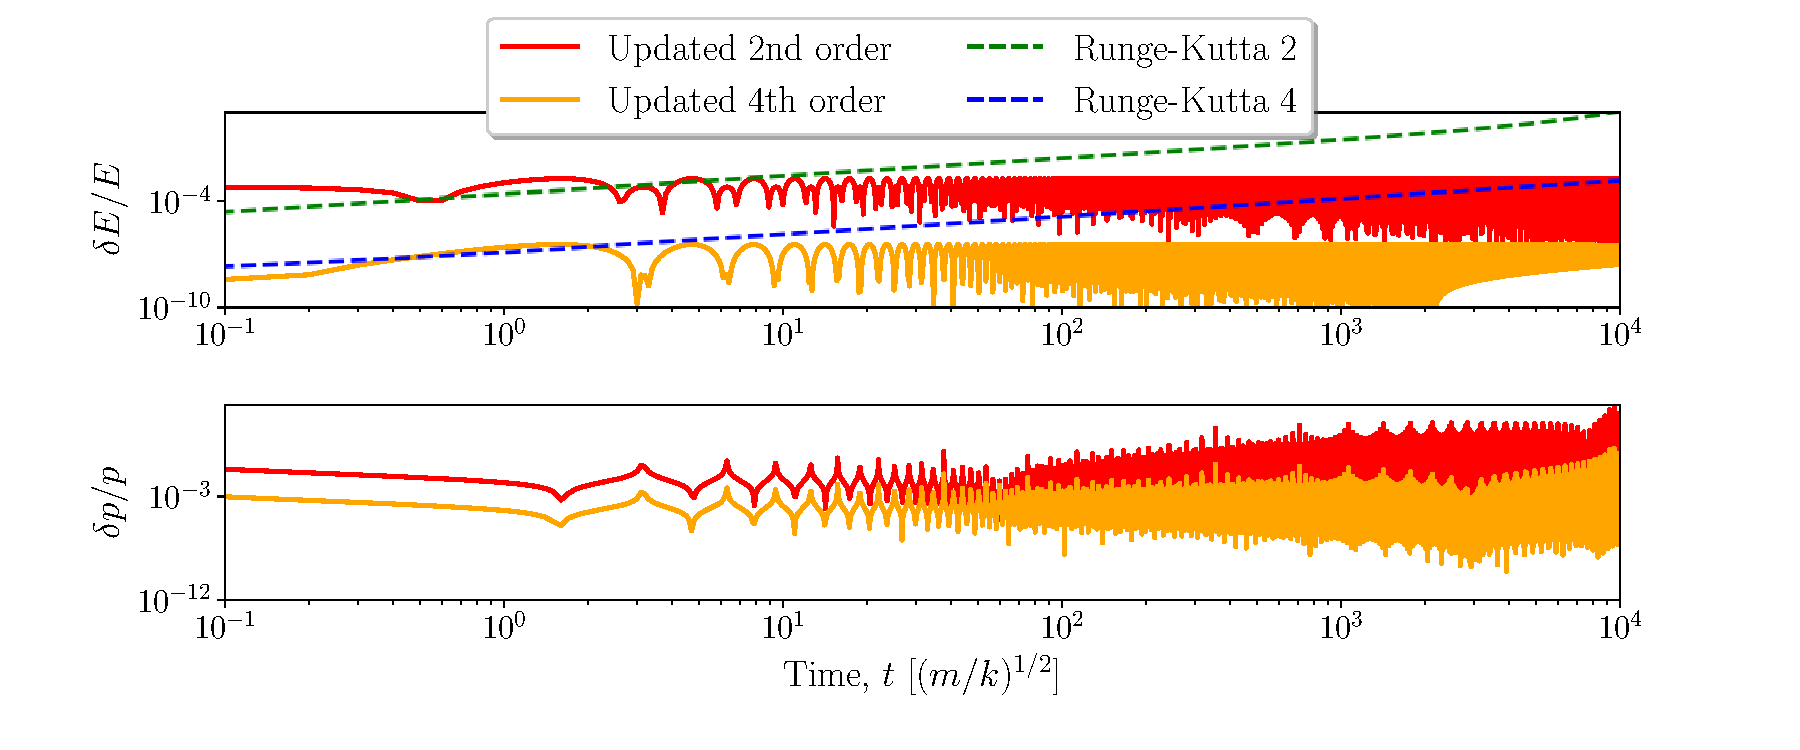
\includegraphics[width=\columnwidth]{figures/dho_energy_momenta_fractional_err.pdf}
  \caption{A comparison of the error in the energy, top, and momenta, bottom, as a fraction of the known analytic solution of the system, of the \updimpl{} simulating a damped harmonic oscillator. One can clearly observe that the fractional energy error is bounded and displays the oscillating behaviour that we expect from previous work, whereas the momenta error does not display such behaviour. This plot is based off its equivalent in the original paper \cite[Figure 2, bottom]{tsangSLIMPLECTICINTEGRATORSVARIATIONAL2015}.}
\end{figure}

As discussed we first verify that the required errors orders are preserved by the \updimpl{} when compared to the \orgimpl{} and traditional non-variational integrators. This can be seen in \fref{fig:dho_energy_bounds} where the fractional error of the system from the true analytic solution is compared directly against the performance of the \orgimpl{} and Runge-Kutta order 2 and 4. We clearly observe that the fractional energy error remains bounded across the timeframe of iteration. This is not the case for the fractional momenta error however as fixed-time-step variational methods such as those implemented cannot be both slimpletic-momentum and momentum-energy preserving \cite{zhongLiePoissonHamiltonJacobiTheory1988}.

% TODO: Fit things to these power laws
\begin{figure}[t]
  \label{fig:dho-n-runtime}
  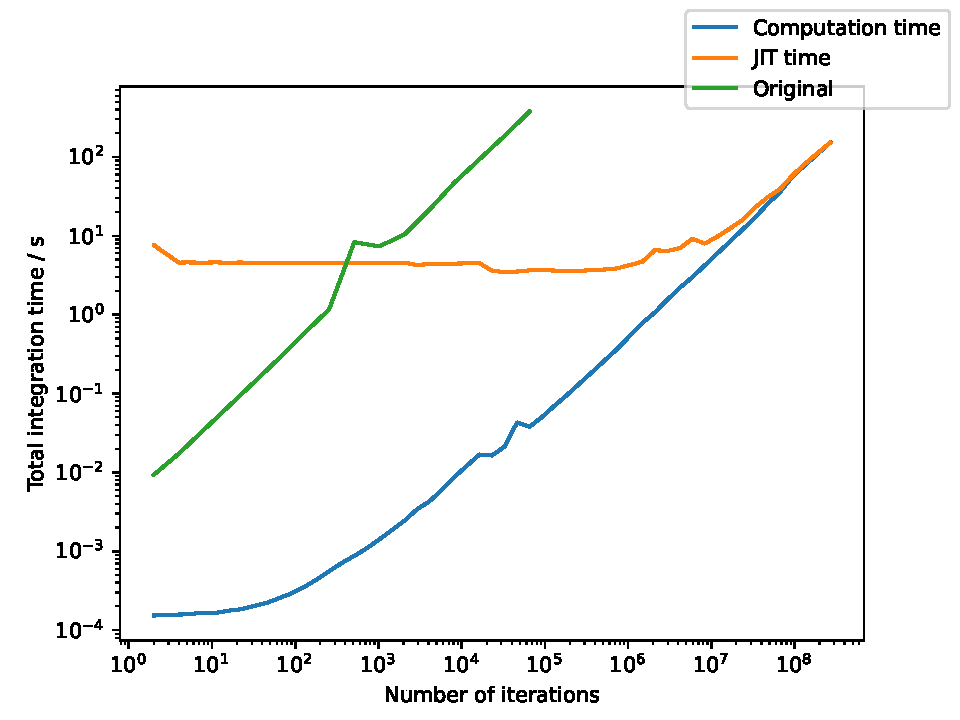
\includegraphics[width=\columnwidth]{figures/dho_n_runtime.pdf}
  \caption{A comparison of running a damped harmonic oscillator system for various numbers of iterations, with $r = 2, \Delta t = 0.1$. The \updimpl{} runtime is split into two components where \enquote{JIT time} represents the one time fixed cost of compiling the function (see \sref{sec:intro-autodiff}) and \enquote{Computation time} represents the actual time spent on computation.
  Each value is a mean of 4 runs, with the \orgimpl{} being cut off early due after $> 20$ minutes runtime for the next sample.}
\end{figure}

\begin{figure}[t]
  \label{fig:dho-r-runtime}
  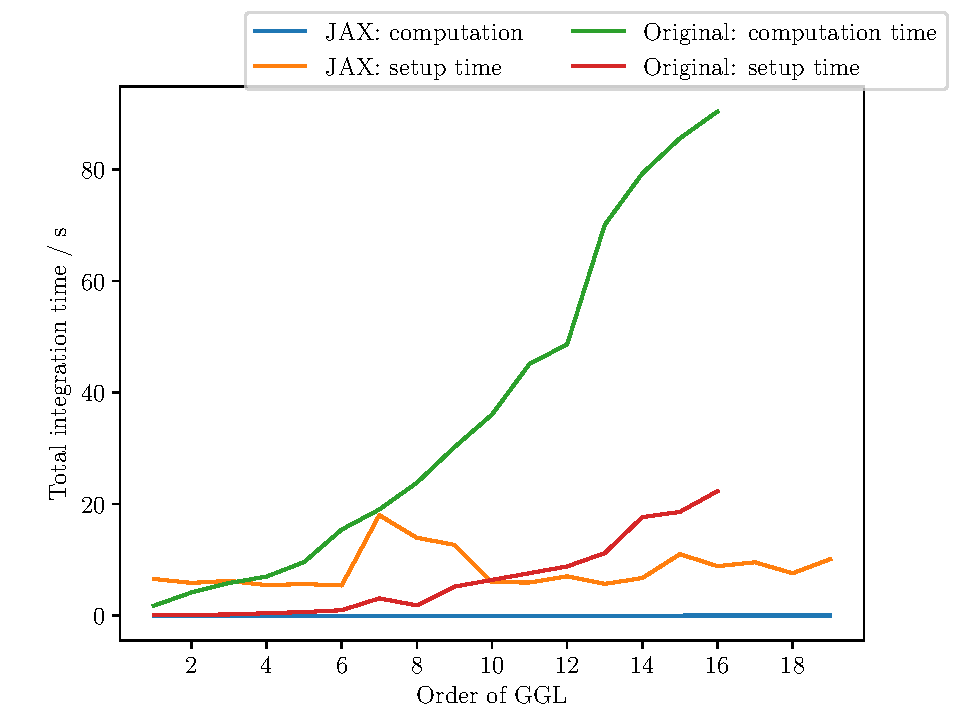
\includegraphics[width=\columnwidth]{figures/dho_r_runtime_linear.pdf}
  \caption{A comparison of running a damped harmonic oscillator system for various values of $r$, the order of the GGL quadrature, with $N_{\mathrm{iter}} = 500, \Delta t = 0.1$ (Apple M1 Max, 64GB of ram).
	For both implementations we split the overall time into setup and computation, each sampled 4 times, as changing the method order requires re-discretising the Lagrangian and thus non-trivial work under both implementations.}
% TODO: Talk about the bump around r=8
\end{figure}

Next we explored the time complexity of the system in terms of the iteration count, $N_{\text{iter}}$ \todo{Define this earlier}, and GGL quadrature order, $r$. These are important to physical applications as they determine the limits of iteration accuracy when iterating over large timescales, error scaling as $(\Delta t)^{2r + 2}$ \todo{check} and total timeframe being $N_{\text{iter}} \Delta t$.

Focusing first on the time complexity in $N_{\text{iter}}$ as shown in \fref{fig:dho-n-runtime}, we note that that the computation time of the \updimpl{} has a much lower starting point as well as scaling factor, growing as TODO, compared the the \orgimpl{}'s TODO. In addition we note that the fixed cost JIT compilation remains roughly constant until growing as a power law from about $10^7$ iterations, where we estimate arrays become greater than 1Gb in size possibly hitting JAX de-optimisation.

This pattern is again seen in \fref{fig:dho-r-runtime} when comparing investigating the time-complexity in the order of the method. Again the JIT time remains roughly constant across the domain tested, and though it starts out initially higher than than the \orgimpl{}'s setup costs, the \orgimpl{}'s computation time quickly swamps this fixed cost. The computation time for the \updimpl{} grows again as a power series, TODO, remaining insignificant in the overall runtime. It should be noted that while increasing the order of the method will increase the precision, at higher orders we start encountering issues with the fixed precision \texttt{float64} type used for calculation in the \updimpl{} compared the the arbitrary precision numerics employed in the \orgimpl{}. Still however this represents an overall improvement in accuracy in physically meaningful simulations as the required precision could be more readily attained by decreasing $\Delta t$ rather than increasing $r$, avoiding the blowup of runtime observed in the \orgimpl{}, or the degradation of precision at high $r$ in the \updimpl{}. The runtime increase observed around $r = 7$ is repeatable and of uncertain origin, we suspect this is due to optimisation cliffs in the JAX internal code as we move between two internal implementations. \todo{Should this be in the general discussion?}

To end the direct application of the \updimpl{} to physical systems we exploit its ability to work on large collections of similar systems, across different choices of physical parameters and initial conditions without incurring the fixed costs discussed prior. To display this we choose to simulate a large collection of double pendulums, with damping on the fixed pendulum, from different initial conditions to observe the chaotic behaviour as seen in \fref{fig:ddp}.

\begin{figure}[t]
  \label{fig:ddp}
  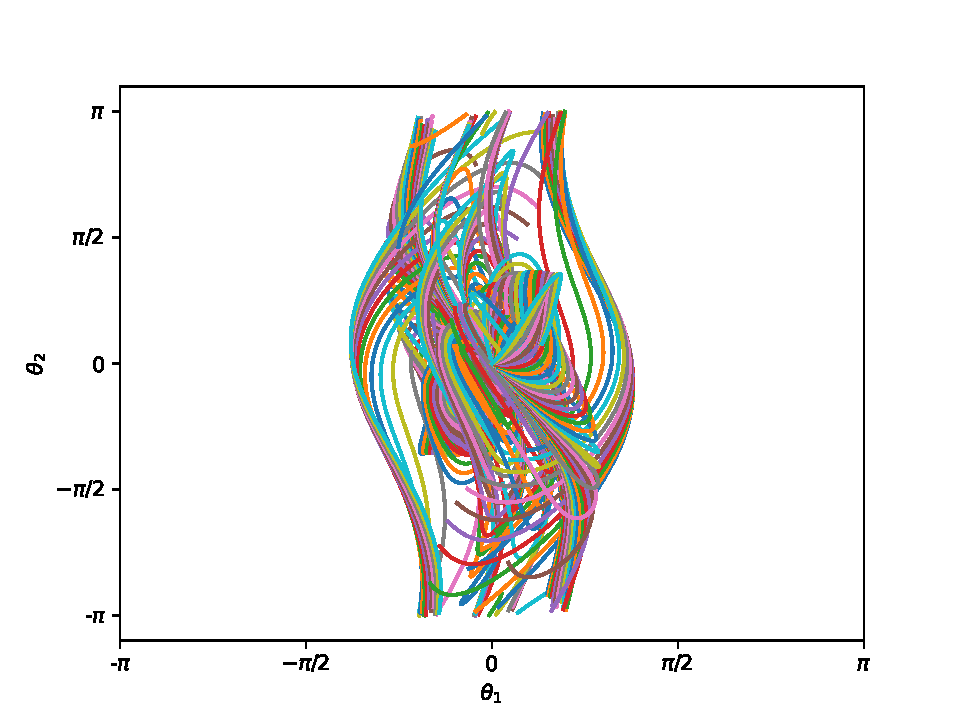
\includegraphics[width=\columnwidth]{figures/damped-double-pendulum.pdf}
  \caption{Phase space plots of $\theta_1$ and $\theta_2$ for a double pendulum, pendulum 1 fixed, and pendulum 2 attached to 1. Both pendulums have uniform densities and unit mass and lengths. The fixed pendulum has damping applied which can be seen by the general spiral inwards over the duration of the lines. TODO: This isnt the cleanest but I want a physical simulation, can I do better?}
\end{figure}

%
%
%\begin{enumerate}
%	\item Modelling of MD system
%	\item PRD? for physics?
%\end{enumerate}

% We got X% speed up
% TODO: This would be good to estimate. This means we can model Y% larger systems for Z% longer time frames

\subsection{Loss Functions}
\label{sec:res-lf}

Moving now onto the loss function and choice Lagrangian embedding. We explored a number of loss functions through a combination of gradient-descent and visual inspection. A wide number of loss functions were tested however focusing on those surrounding systems of harmonic oscillators, we settled on a number as shown in \tref{table:embeddings}. These were paired with a number of simple loss functions, \tref{table:loss-fns}, drawing from physical knowledge and previous work on loss functions connected to neural networks.

These were chosen as system specific embeddings as good candidates for exploration of the embedding space. By performing gradient descent we were able to obtain matches for a number of random initial embeddings \todo{do this and put it in a table} as shown in \tref{table:optimisation-results}. From this data we aimed to determine empirically the suitability of optimisation within the embedding space under a given loss function, as a strictly simpler problem than computing it for a compose neural network.

An example of the behaviour of one combination of loss function and embedding can be seen in \fref{fig:loss-fn-plots}, here we see around the successfully attained minima after optimisation that the loss is indeed in all but one \todo{check this still holds for the one that we choose} dimension. This suggests that while the loss function is not ideal, it does provide a somewhat suitable space in which to optimise.

From these attempts we were able to determine that

\begin{itemize}
  \item Prefactor helped it not get stuck, introduced redundancy
  \item Often explode to infinity and thus want to wait against that
\end{itemize}


\begin{table}
\label{table:embedding-choices}
\caption{A list of em}
\begin{tabular}{l|c|c|c}
  Name & Space & $L$ & $K$ \\
  \hline
  SHM & $(m, k) \in \R^2$ & $\frac 12 m \dot \vbq^2 + \frac 12 k \vbq^2$ & 0 \\
  SHM + prefactor & $(m, k, \alpha) \in \R^3$ & $\alpha(\frac 12 m \dot \vbq^2 + \frac 12 k \vbq^2)$ & 0 \\
  DHO & $(m, k, \lambda) \in \R^3$ & \\
  DHO + prefactor & $(m, k, \lambda, \alpha) \in \R^3$
\end{tabular}
\end{table}

\begin{table}
\label{table:loss-fns}
\caption{A list of loss functions. RMS = Root Mean Squared, a standard loss function.}
\begin{tabular}{l|c|c|c}
  Name & Space & $L$ & $K$ \\
  \hline
  RMS both \\
  DHO \\
  DHO + prefactor \\
\end{tabular}
\end{table}

\begin{table}
\label{table:optimisation-results}
\caption{A list of loss functions. RMS = Root Mean Squared, a standard loss function.}
\begin{tabular}{l|c|c|c}
  Name & Space & $L$ & $K$ \\
  \hline
  RMS both \\
  SHM + prefactor  \\
  DHO \\
  DHO + prefactor \\
\end{tabular}
\end{table}


\subsection{PINN and Approximating Damped Harmonic Oscillators}

%\begin{enumerate}
%  \item x $5.0 × 10^5$ random embeddings
%  \item x DHO
%  \item x Physical domain
%  \item x 5pc set to zeroes
%  \item x Negative values penalised
%  \item x Training tempermental
%		Josh: non-convexity?
%  \item x The model produced a RMS error value of X Y for Q PI.
%  \item x The loss functionwas also varied during the training process,
%  \item x initially weighting more in favour of the RMS error in q to compensate for the fact that a majorityof systems produced larger π-values than q-values.
%  \item x Other things attempted: trying only pi, this prodcued things with $m \approx k \approx \lambda$
%  \item Often ended up with values of roughly correct proportion implying that the 4 parameter emebdding may have been useful
%\end{enumerate}


Finally we applied these techniques to an PINN. For our initial explorations in this space we focused on fitting to systems of damped harmonic oscillators as has been the through line of the work thus far. We chose the 3 parameter DHO embedding over the 4 parameter embedding with a pre-factor as while it was more effective when subject to direct gradient descent, we were concerned that the additional redundant embedding parameter would make learning the systems more complex and error prone. 

The dataset used ($N \approx 5 \times 10^5$) in training was a mixed selection, primarily it was comprised of uniformly distributed embeddings within the subset of the physical region of the embedding space (positive embedding values). In addition a fraction, approximately $5 \%$ for each, of the spring and damping constants were set to zero to ensure that the model was exposed to SHM and kinetic only systems.

For PINN training, accounting for the increased complexity of the optimisation problem now being with respect to the parameters of the model, we made two alterations to our loss functions. First we added a strong weight against non-physical negative embedding values in our loss function, taking the form of,

\begin{equation}
  f(e_i) = \begin{cases}
  	0 & e_i \ge \delta \\
  	\exp{-\gamma e_i} & e_i < \delta 
  \end{cases}
\end{equation}

where $\delta = −0.1$ is a tolerance to allow for zero to be a non-penalised output and $\gamma \approx 10$ is the strength of the penalisation. In addition we also experimented with capping the values of the loss at large values to mitigate overflows when dealing with particularly bad fits, such as the initially random initialised weights before any training had commenced.

Model training was done in batches and was prone to explosion possible due to the non-convexity in some regions as discussed in \sref{sec:res-lf}. Overall it was found that training could be made more stable by increasing batch sizes to $512$ and manually tweaking loss weightings (for example between the $\vb q$ and $\pi$ RMS terms where more progress was made with weighting towards $\vbq$ error to counteract observed larger tendency for error in this term) and learning rates as training progressed \todo{want to talk about learning rate in the NN or LF prelim section}. 

Other loss functions, such as RMS in $\pi$ only were investigated producing good losses on the order of $10^{-4}$, however on later inspection it was found that these resulted from a finding a false minima of $m \approx k \approx \lambda$, highlighting the complexity of the embedding space in representing physical systems.

By the training's conclusion we obtained an RMS error of $\pm 5 \times 10^{-2}$ in $\vbq$ and $\pm 1 \times 10 ^{-1}$ in $\pi$. This model was able to predict systems with some accuracy, clearly able to fit to certain features as shown in \fref{fig:model-prediction}.

We often observed predicted embeddings with values of roughly correct proportion, but off some some constant factor, implying that the 4 parameter embedding or other normalisation method may have been useful as the system was unable to move past this local minima in phase space, representing a sufficiently similar physical system. \todo{I should mention this similarity in the}

\begin{figure}[t]
  \label{fig:model-prediction}
  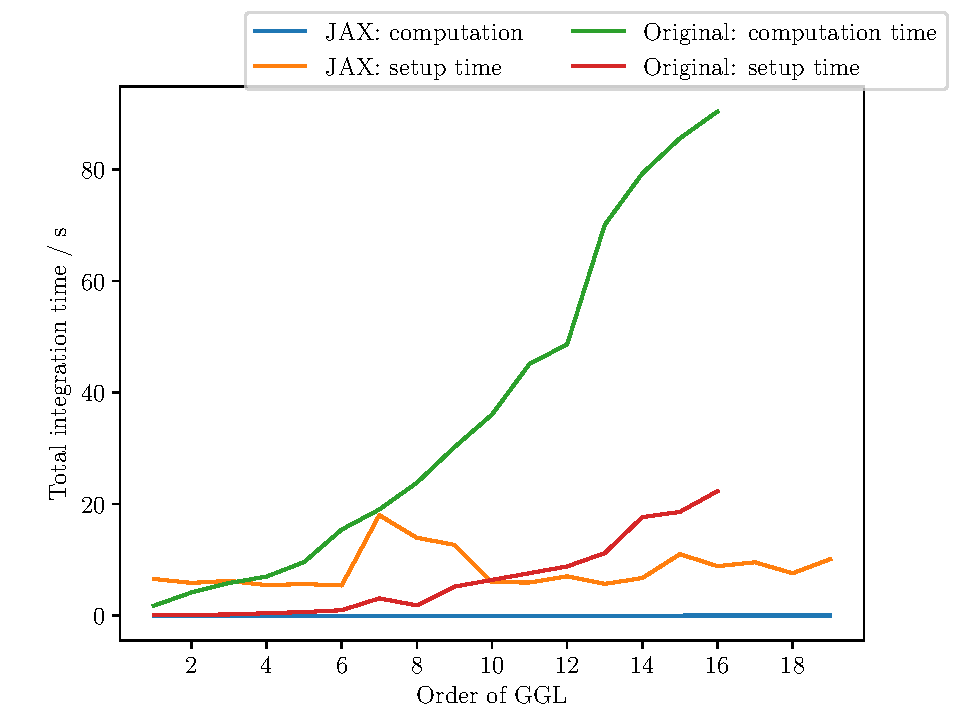
\includegraphics[width=\columnwidth]{figures/dho_r_runtime_linear.pdf}
  \caption{A comparison of the behaviour of a predicted Lagrangian embedding from the PINN. True embedding, $(TODO)$, predicted embedding $(TODO)$}
\end{figure}

\section{General Discussion}

% What do the pretty graphs actually mean in a broad sense
% Pull together with the background
% PHYSICS!!!

% Talk about the redundancy in neural networks

% Is this where we will mention the "future work" of NNs?

\section{Conclusion}
